\documentclass[svgnames,11pt]{beamer}
\input{/home/tof/Documents/Cozy/latex-include/preambule_commun.tex}
\input{/home/tof/Documents/Cozy/latex-include/preambule_beamer.tex}
%\usepackage{pgfpages} \setbeameroption{show notes on second screen=left}
\author[]{Christophe Viroulaud}
\title{Exercice interblocage\\Le dîner des philosophes}
\date{\framebox{\textbf{Archi 09}}}
%\logo{}
\institute{Terminale - NSI}
%DODO voir exo 2 du concours général sujet 0
\begin{document}
\begin{frame}
\titlepage
\end{frame}
\begin{frame}
    \frametitle{}

    Le \emph{dîner des philosophes} est un problème présenté par  Edsger Dijkstra.
La situation est la suivante :
\begin{itemize}
\item cinq philosophes se trouvent autour d'une table ;
\item chacun des philosophes a devant lui un plat de spaghetti ;
\item à gauche de chaque plat de spaghetti se trouve une fourchette.
\end{itemize}
\begin{center}
\centering
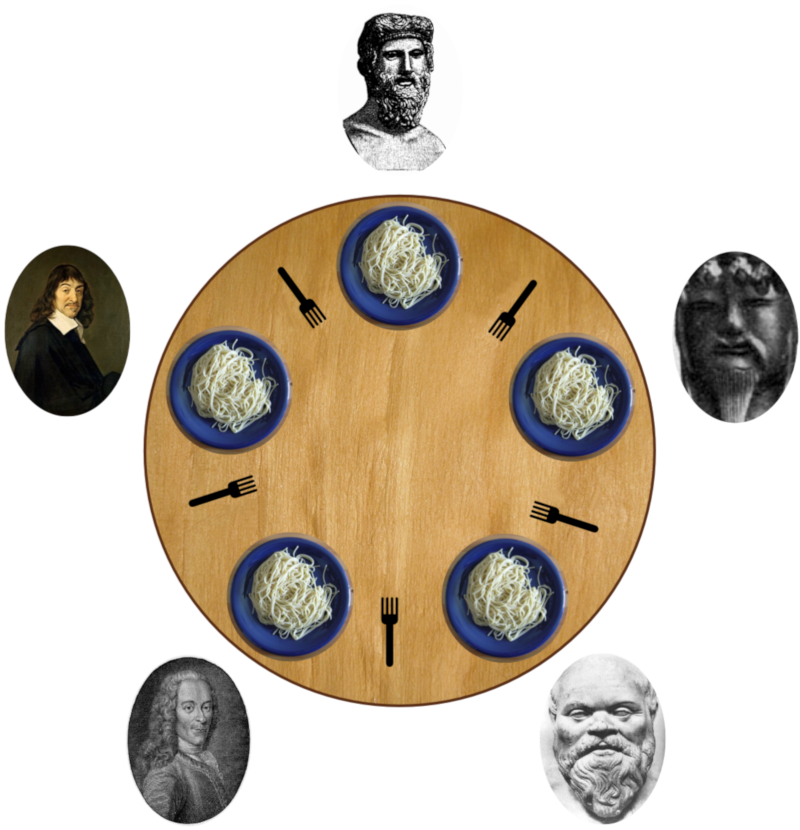
\includegraphics[width=4cm]{ressources/philo.png}
\captionof{figure}{dîner des philosophes}
\label{IMG}
\end{center}
\end{frame}
\begin{frame}
    \frametitle{}

    Un philosophe n'a que trois états possibles :
\begin{itemize}
\item penser pendant un temps indéterminé ;
\item être affamé (pendant un temps déterminé et fini sinon il y a famine) ;
\item manger pendant un temps déterminé et fini.
\end{itemize}

\end{frame}
\begin{frame}
    \frametitle{}

    Des contraintes extérieures s'imposent à cette situation :
\begin{itemize}
\item quand un philosophe a faim, il va se mettre dans l'état « affamé » et attendre que les fourchettes soient libres ;
\item pour manger, un philosophe a besoin de deux fourchettes : celle qui se trouve à gauche de sa propre assiette, et celle qui se trouve à droite (c'est-à-dire les deux fourchettes qui entourent sa propre assiette) ;
\item si un philosophe n'arrive pas à s'emparer d'une fourchette, il reste affamé pendant un temps déterminé, en attendant de renouveler sa tentative.
\end{itemize}

\end{frame}
\begin{frame}
    \frametitle{}

    \begin{activite}
    \begin{enumerate}
        \item Rappeler les conditions d'interblocage.
        \item Montrer alors que le dîner des philosophes peut conduire à une situation d'interblocage.
    \end{enumerate}
    \end{activite}

\end{frame}
\begin{frame}
    \frametitle{Avant de regarder la correction}
\begin{center}
    \centering
    \includegraphics[width=3cm]{/home/tof/Documents/Cozy/latex-include/stop.png}
    \end{center}
{\Large
    \begin{itemize}
        \item Prendre le temps de réfléchir,
        \item Analyser les messages d'erreur,
        \item Demander au professeur.
    \end{itemize}
}
\end{frame}
\begin{frame}
    \frametitle{Correction}

Dans le dîner des philosophes, les quatre conditions de Coffman sont satisfaites:
\begin{itemize}
\item Les ressources sont \textbf{en accès exclusif}: deux philosophes ne peuvent pas utiliser la même fourchette en même temps.
\item \textbf{Rétention et attente}: chaque philosophe prend la fourchette de gauche et attend celle de droite.
\item \textbf{Non préemption}: un philosophe ne peut pas prendre une fourchette dans les mains d'un autre.
\item \textbf{Attente cyclique}: chaque philosophe attend la fourchette (occupée) à sa droite.
\end{itemize}

\end{frame}
\end{document}
